
In this document, we propose an IVOA standard data model (DM) for describing the provenance of astronomical data. 
How this specification of the Provenance model can be implemented is developed in a companion document to be published as an IVOA Note \citep{std:ProvenanceImplementationNote}.

The provenance of scientific data is cited in the FAIR principles for data sharing \citep{FAIR-principles}.
Provenance is relevant for science data in general and specifically in an open publishing context which is a requirement for many
projects and collaborations.
% and corresponds to particularly relevant information in the context of openly published science data.

We follow the definition of provenance as proposed by the W3C \citep{std:W3CProvDM}, i.e.~that provenance is ``information about entities, activities, and people involved in producing a piece of data or thing, which can be used to form assessments about its quality, reliability or trustworthiness''.

In astronomy, such entities are generally datasets composed of VOTables, FITS files, database tables or files containing values (spectra, light curves),  it could also be any value, logs, documents, as well as physical objects such as instruments, detectors or photographic plates.
The activities correspond to processes like an observation, a simulation, processing steps (image stacking, object extraction, etc.), execution of data analysis code, publication, etc.
The people involved can be for example individual persons (observer, publisher, etc.), groups or organisations, i.e.~any agent related to an activity or an entity.

An example for activities, entities and agents as they can be discovered backwards in time is given in Figure~\ref{fig:example-workflow}.


\begin{figure}[ht]
\centering
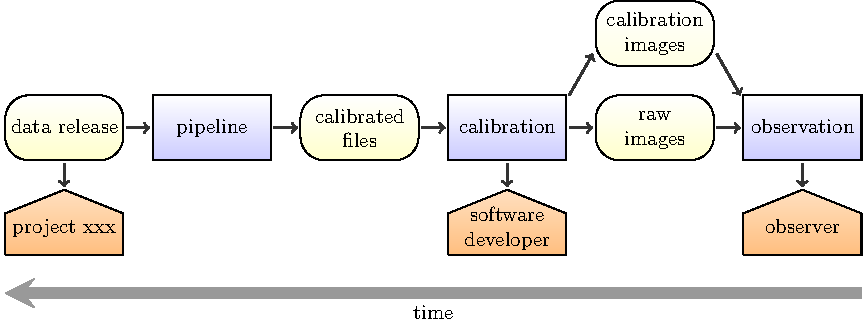
\includegraphics[width=1\textwidth]{workflow-backwards.pdf}
\caption[Example graph of provenance discovery]{An example graph of provenance discovery. Starting with a released dataset (left), the involved activities (blue boxes), 
progenitor entities (yellow rounded boxes) and responsible agents (orange pentagons) are 
discovered.}
\label{fig:example-workflow}
\end{figure}


\subsection{Goal of the provenance model}
\label{sec:goals}

The goal of this Provenance DM is to describe how provenance information arising from astronomy projects can be modelled, stored and exchanged. 
Its scope is mainly modelling of the flow of data, of the relations between pieces of data, and of processing steps. 
However, the Provenance DM is sufficiently abstract that its core pattern could be applied to any kind of process related to either observation or simulation data.

Information attached to observation activities such as ambient conditions and instrument characteristics provide useful information to assess the quality and reliability of the generated entities.
Contextual information during the execution of processing activities (computer structure, nodes, operating system used, etc.) can also be relevant for the description of the main entities generated. 
This complementary information should be included in the form of metadata or additional entities connected to an activity. 
However, the precise structure and modelling of this information is out of the scope of this document. 

In general, the model shall capture information in a machine-readable way that would enable a scientist who has no prior knowledge about a dataset to get more background information. 
This will help the scientist to decide if the dataset is adequate for her research goal, assess its quality and reliability and get enough information to be able to trace back its history as far as required or possible. 

Provenance information can be exposed with different granularity. A specific project has to decide this granularity.
The granularity and amount of provenance information provided depends on the available information, the needs of the project and the intended usage of this information.

This flexible approach has an impact on the interoperability between different services as this level of detail is not known a priori. 
The objective of the model is to propose a general structure for the provenance information. In addition, proposed vocabularies of reserved words help to further formalize the detailed provenance information.


The following list is a collection of use cases addressed by the Provenance DM. 


\paragraphlb{A: Traceability of products}
        Track the lineage of a product back to the raw material (backwards search), show the
        workflow or the data flow that led to a product.

        \noindent Examples: 
        \begin{itemize}
            \item Having a dataset, find the main progenitors and in particular locate the raw data.
            \item Find out what processing steps have been already performed for a given dataset: Is an image already calibrated? What about dark field subtraction? Were foreground stars removed?
            \item Find out if a filter to remove atmospheric background muons has been applied.
        \end{itemize}


\paragraphlb{B: Acknowledgement and contact information}
        Find the people involved in the production of a dataset, the people\slash{}organizations\slash{}institutes that one may want to acknowledge or can be asked for more information.

        \noindent Examples: 
        \begin{itemize}
            \item I want to use an image for my own work -- who was involved in creating it? Who can I contact to get information? 
            \item Who was on shift while the data was taken?
            \item I have a question about column xxx in a data table. Who can I ask about that? 
        \end{itemize}


\paragraphlb{C: Quality and Reliability assessment}
Assess the quality and reliability of an observation, production step or dataset, e.g., based on detailed descriptions of the processing steps and manipulated entities.
        
        \noindent Examples:
        \begin{itemize}
            \item Get detailed information on the methods/tools/software that were involved: What algorithm was used for Cherenkov photon reconstruction? How was the stacking of images performed?
            \item Check if the processing steps (including data acquisition) went ``well'': Were there any warnings during the data processing? Any quality control parameters?
            \item Extract the ambient conditions during data acquisition (cloud coverage? wind? temperature?)
            \item Is the dataset produced or published by a person/organisation I rely on? Using methods I trust?
        \end{itemize}


\paragraphlb{D: Identification of error location}
Find the location of possible error sources in the generation of a product. This is connected to use cases described in section C above, but implies an access to more information on the execution such as configuration or execution environment.

        \noindent Examples:
        \begin{itemize}
            \item I found something strange in an image. Was there anything strange noted when the image was taken? a warning during the processing? 
            \item Which pipeline version was used, the old one with a known bug for treating bright objects or a newer version? 
            \item What was the execution environment of the pipeline (operating system, system dependencies, software version, etc.)?
            \item What was the detailed configuration of the pipeline? were the parameters correctly set for the image cleaning step?
        \end{itemize}


\paragraphlb{E: Search in structured provenance metadata}
        Use Provenance criteria to locate datasets (forward search), e.g., finding all images produced by a certain processing step or derived from data which were taken by a given facility.
        
        \noindent Examples:
        \begin{itemize}
            \item Find more images that were produced using the same version of the CTA pipeline.
            \item Get an overview of all images reduced with the same calibration dataset.
            \item Are there any more images attributed to this observer?  
            \item Find all datasets generated using this given algorithm, with this given configuration, for this given step of the data processing.
            \item Find all generated data files that used incorrectly generated file X as an input, so that they can be marked for re-processing
            \item Extract all the provenance information of a SVOM light curve or spectrum to reprocess the raw data with refined parameters.
        \end{itemize}

\paragraphlb{General Remarks}
In addition to those use cases, if the stored information is sufficiently fine grained, it is possible to enable the \textbf{reproducibility} of an activity or sequence of activities, with the exact same configuration and exact same conditions.

Provenance information delivers additional information about a scientific dataset to enable the scientist to evaluate its \textbf{relevance for his work}.
